%%%%%%%%%%%%%%%%%%%%%%%%%%%%%%%%%%%%%%%%%%%%%%%%%%%%%%%%%%%%%%%%%%%%%%%%%%%%%%%%
%2345678901234567890123456789012345678901234567890123456789012345678901234567890
%        1         2         3         4         5         6         7         8
\documentclass[letterpaper, 10 pt, conference]{IEEEtran}
%{\documentclass[letterpaper, 10 pt, conference]{ieeeconf}%}  % Comment this line out
                                                          % if you need a4paper
%\documentclass[a4paper, 10pt, conference]{ieeeconf}      % Use this line for a4
                                                          % paper

\IEEEoverridecommandlockouts                              % This command is only
                                                          % needed if you want to
                                                          % use the \thanks command

% See the \addtolength command later in the file to balance the column lengths
% on the last page of the document



% The following packages can be found on http:\\www.ctan.org
%\usepackage{graphics} % for pdf, bitmapped graphics files
%\usepackage{epsfig} % for postscript graphics files
%\usepackage{mathptmx} % assumes new font selection scheme installed
%\usepackage{times} % assumes new font selection scheme installed
%\usepackage{amsmath} % assumes amsmath package installed
%\usepackage{amssymb}  % assumes amsmath package installed

\usepackage{graphicx}

% Keywords command
\providecommand{\keywords}[1]
{
  \small	
  \textbf{\textit{Keywords---}} #1
}


\title{\LARGE \bf
Load Balancing Using SDN
}

\author{\IEEEauthorblockN{Anand Wani\IEEEauthorrefmark{1},
Bhavik Dhandhalya\IEEEauthorrefmark{2}, Prof. Virendra Shekhawat\IEEEauthorrefmark{3}}
\IEEEauthorblockA{Computer Science \& Information Systems, Birla Insitute of Technology \& Science, Pilani, IND.\\
Email: \IEEEauthorrefmark{1}h20180143@pilani.bits-pilani.ac.in,
\IEEEauthorrefmark{2}h20180118@pilani.bits-pilani.ac.in,
\IEEEauthorrefmark{3}vsshekhawat@pilani.bits-pilani.ac.in}}

\begin{document}



\maketitle
\thispagestyle{empty}
\pagestyle{empty}


%%%%%%%%%%%%%%%%%%%%%%%%%%%%%%%%%%%%%%%%%%%%%%%%%%%%%%%%%%%%%%%%%%%%%%%%%%%%%%%%
\begin{abstract}

 Traditional networks find it difficult to cope up to the demands of the current applications. SDN addresses this issue by decoupling the control and data planes. Software Defined Network is new network technology which is increasing functionality of networks by making it programmable and vendor neutral. Our Network should be flexible to handle large amount of traffic. In this project we aim to implement an efficient load balancing technique. Here we have analysed and compared the performance of random, round-robin, least connection based strategy and weighted round-robin for balancing the load on the servers using SDN framework want to use it if say you.


\end{abstract}

\begin{IEEEkeywords}
Software Defined Networks, Load Balancing, Round Robin. 
\end{IEEEkeywords}

%%%%%%%%%%%%%%%%%%%%%%%%%%%%%%%%%%%%%%%%%%%%%%%%%%%%%%%%%%%%%%%%%%%%%%%%%%%%%%%%
\section{Introduction}
\label{sec:intro}

Software Defined Networking (SDN) is the network architecture approach where network control is separated from forwarding plane (data plane) and is directly programmable ~\cite{c1}. SDN model consists of infrastructure layer which consists of switching devices. This layer is responsible for forwarding and data processing capabilities of the network. Next layer of SDN architecture is control layer. It acts as a interface between infrastructure layer and application layer.  Control plane is the logical entity that receives instructions or requirements from the SDN Application layer and relays them to the networking components. The control layer also extracts information about the network from the hardware devices and communicates back to the SDN Applications with an abstract view of the network, including statistics and events about what is happening. The application layer consists of SDN application, that is designed to fulfil requirement of user. This layer is residing above the control layer. OpenFlow protocol used in SDN helps in communication of control plane with data plane. The brain of network is implemented in the software called controller. The intelligence or the logic of where and how to make forwarding is residing in control plane. An OpenFlow switch consists of one or more flow tables consisting of rules stating actions to be taken for the incoming packets. Incoming packet is matched against value of rule that are stored in flow tables necessary actions are taken. ~\cite{c4} Actions can be either to drop that packet, forward to controller or forward by normal pipeline processing. On the nature of rules installed, an OpenFlow switch can behave like a switch, firewall, Load balancer, router etc. Fig. 1. highlights the SDN architecture. This project aims at performing load balancing on the servers using various strategies in the SDN network infrastructure ~\cite{c2} Various strategies used for load balancing are Random, Round Robin, Weighted Round Robin and Least connection based strategy. 

\begin{figure}[ht!]
\centering
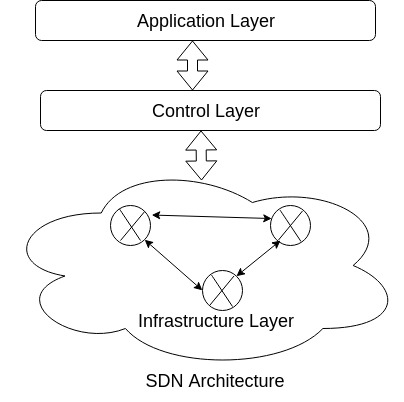
\includegraphics[width=\linewidth]{SDN.jpeg}
\caption{SDN Architecture \label{fig:1}}
\end{figure}


%{\section{PROCEDURE FOR PAPER SUBMISSION}%}
\section{System Model}
\label{sec:system model}
%{\subsection{Selecting a Template (Heading 2)}%}
%{\subsection{Maintaining the Integrity of the Specifications}%}

Consider a system in which there are M servers and a single controller for load balancing and distribution on these servers. There are N  clients wanting server CPU time and other resources.


\begin{figure}[ht!]
\centering
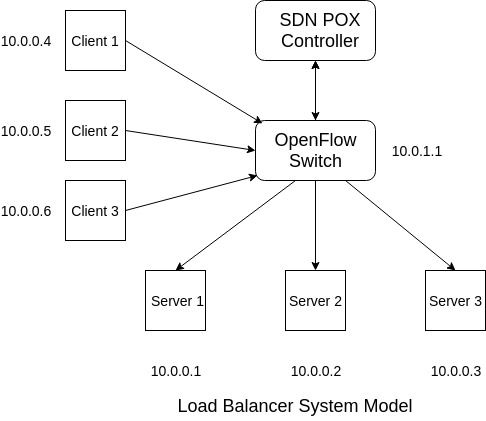
\includegraphics[width=\linewidth]{SystemModel.jpg}
\caption{System Model \label{fig:2}}
\end{figure}


\section{PROPOSED STRATEGY}
In this section, we have presented various strategies used for solving the load balancing problem.


\subsection{Random Strategy}
As its name suggests, this algorithm selects a server on random basis, i.e. using an underlying random number generator. In cases wherein the load balancer receives a large number of requests, a Random algorithm will be able to distribute the requests evenly to the nodes. So like Round Robin, the Random algorithm is sufficient for clusters consisting of nodes with similar configurations (CPU, RAM, etc). 


\subsection{Round Robin Strategy}

Round Robin is the most widely used algorithm. It is  easy to implement and easy to understand. 
In Random strategy, while user requests come to controller it randomly selects one of the available servers ~\cite{c3}. But in round-robin fashion, it tries to distribute load uniformly to all servers. Results show that Round-robin is better than Random strategy in terms of response time, latency and throughput.
Let's say we have 2 servers waiting for requests behind the load balancer. Once the first request arrives, the load balancer will forward that request to the 1st server. When the 2nd request arrives, that request will then be forwarded to the 2nd server.
Because the 2nd server is the last in this cluster, the next request (i.e., the 3rd) will be forwarded back to the 1st server, the 4th request back to the 2nd server, and so on, in a cyclical fashion.

\begin{figure}[ht!]
\centering
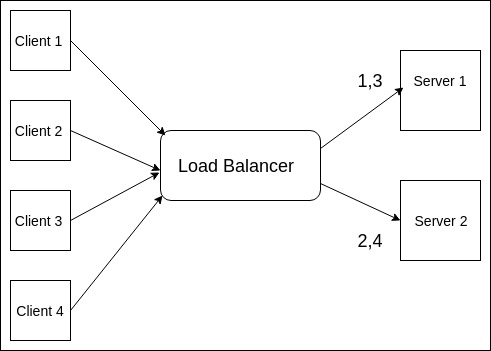
\includegraphics[width=\linewidth]{RR.jpg}
\caption{Round Robin Load Balancer \label{fig:3}}
\end{figure}

Even though this method is simple to implement, it has some limitations, For example, if Server 1 has more CPU, RAM, and other specs compared to Server 2, then Server 1 will be able to handle a higher workload than Server 2. Unfortunately, a load balancer running on a round robin algorithm won't be able to treat the two servers accordingly. In spite of the two servers' disproportionate capacities, the load balancer will still distribute requests equally. As a result, Server 2 can get overloaded faster and probably even go down. The Round Robin algorithm is best for clusters consisting of servers with identical specs.

\subsection{Weighted Round Robin Strategy}

In this approach we can differentiate between heterogeneous servers. Example, if Server 1 is having higher specs than Server 2, the algorithm  will assign more requests to the server with a higher capability of handling load. This algorithm is called as Weighted Round Robin ~\cite{c2}. 
The Weighted Round Robin is similar to the Round Robin in a sense that the requests are assigned to the servers in cyclical manner only, but with a twist. The server with the higher specs will be assigned a greater number of requests ~\cite{c5}. Here when we set up the load balancer, we assign "weights" to each node. The node with the higher specs will be given the higher weight. Weights are in  proportion to actual capacities. For example, if Server 1's capacity is 2x more than Server 2's, then server 1 is assigned a weight of 2 and Server 2 is assigned a weight of 1.

\begin{figure}[ht!]
\centering
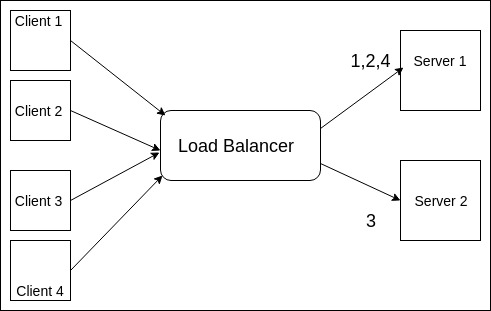
\includegraphics[width=\linewidth]{WRR.jpg}
\caption{Weighted Round Robin \label{fig:4}}
\end{figure}

So when clients requests arrive, the first 2 client request will be assigned to server 1 and the 3rd to server 2. If more clients come in, the same sequence will be followed. That is, the 4th, 5th, 7th, 8th will all go to Server1, and the 6th to Server 2, and so on. 
Capacity isn't the only basis for choosing the Weighted Round Robin (WRR) algorithm. Sometimes, if you want server one to get a substantially lower number of connections than an equally capable server for the reason that the first server is running business critical applications and you don't want it to be easily overloaded. 



\subsection{Least Connections}

Consider an instance where, even if two servers in a cluster have exactly the same specs, one server can still get overloaded considerably faster than the other. The possible reason for this to happen is because clients connecting to Server 2 stay connected much longer than those connecting to Server 1. This can cause the total current connections in Server 2 to pile up, while those of Server 1 with clients connecting and disconnecting over shorter times, would virtually remain the same. As a result, Server 2's resources can run out faster.  
In such a situations, the Least Connections algorithm is a better fit. This algorithm takes into consideration the number of current connections each server has. When a client attempts to connect, the load balancer will try to determine which server has the least number of connections and then assign the new connection to that server.

\section{EXPERIMENTS}
\label{sec:EXPERIMENTS}

We have used mininet for simulating the network. We created the topology as shown in the system model, it has 6 hosts, one SDN switch and one SDN  controller. Controller used is the POX Controller. Protocol used is openflow. 3 hosts are servers and remaining are clients. Servers are running HTTP server application and clients are requesting files of various sizes from the servers.  
Client program also logs the response time for each GET request. This response time is used for plotting graphs and comparing the response time for various approaches.


\section{OBSERVATIONS}
\label{sec:OBSERVATIONS}
In this sections, we present our observations with the help of various graphs.

\subsection{Round Robin And Random}
In this case all servers are of equal configuration, so weights are same, here we have compared the response time, for 100 requests from 3 hosts for different file sizes. The graph shows that the average response time for  each file size is less that is better in case of Round Robin that random strategy. 
The Table. 1.  shows, the average response time of different file sizes for Round Robin and Random strategy.

\begin{figure}[ht!]
\centering
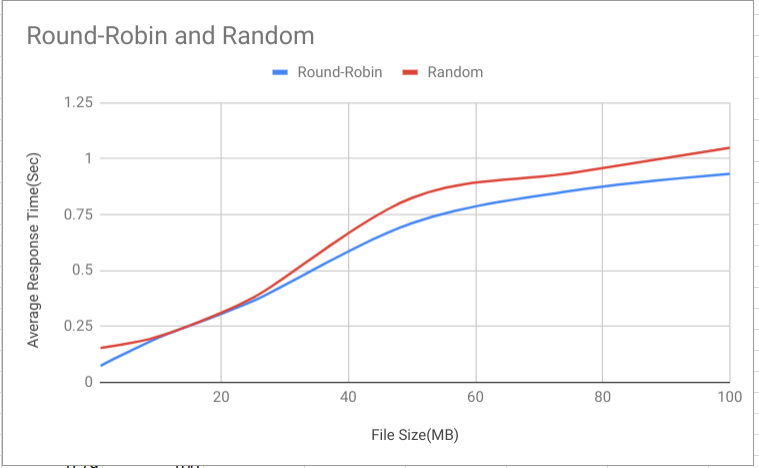
\includegraphics[width=\linewidth]{0.png}
\caption{Round Robin and Random\label{fig:5}}
\end{figure}

\subsection{Weighted Round Robin, Round Robin and Random}
In real world networks, all servers are not identical in terms of specifications, so we have assigned weights to each server based on its capacity to process requests. Based on these weights the controller will insert flow rules in the switch, so that server with higher weight will get more client requests. 
We have used link delays for simulating servers of different configurations. We test this case for various iterations and in each iteration for various file sizes, then plotted graphs of response time vs file size.

\begin{figure}[ht!]
\centering
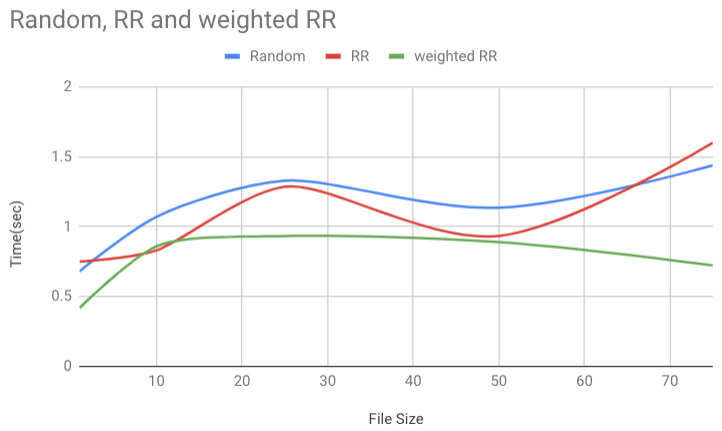
\includegraphics[width=\linewidth]{1.png}
\caption{Round Robin, Random and Weighted Round Robin, 50 File Requests per client \label{fig:6}}
\end{figure}

\begin{figure}[ht!]
\centering
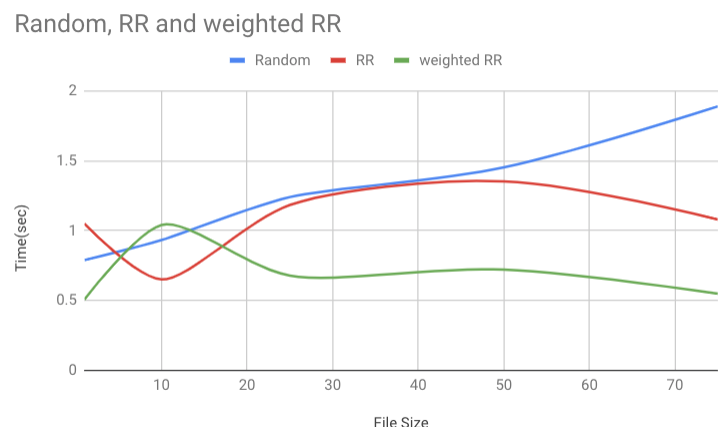
\includegraphics[width=\linewidth]{2.png}
\caption{Round Robin, Random and Weighted Round Robin, 100 File Requests per client \label{fig:7}}
\end{figure}

\begin{figure}[ht!]
\centering
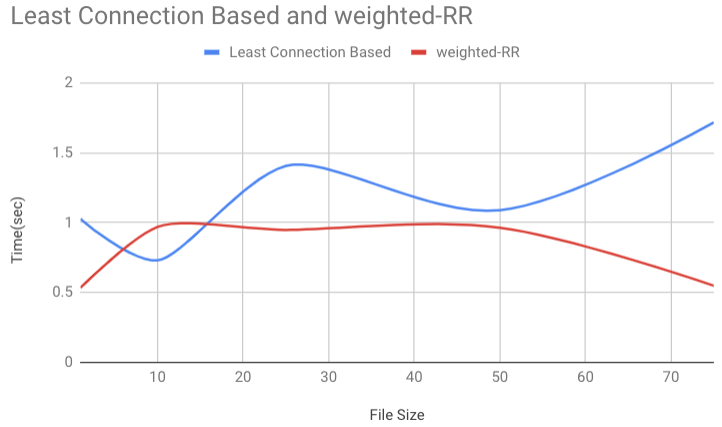
\includegraphics[width=\linewidth]{5.png}
\caption{Least Connection Based and Round Robin \label{fig:9}}
\end{figure}

\subsection{Comparison based on Turn around time}

According to fig. 9 weighted-RR is performing better than random and traditional RR even when packets/files were having different size. During these implementation we have assumed that we know either link delay or server capacity and based on that we have fixed threshold. The relation between server capacity and threshold is still an open question. If one can find the threshold manually and fix it, then we can have enormous performance advantage over any other algorithms as shown in fig. 10. In fig. 10 we have considered only similar sized packets and we have fixed the threshold manually. That manual threshold lead us to enormous performance.

\begin{figure}[ht!]
\centering
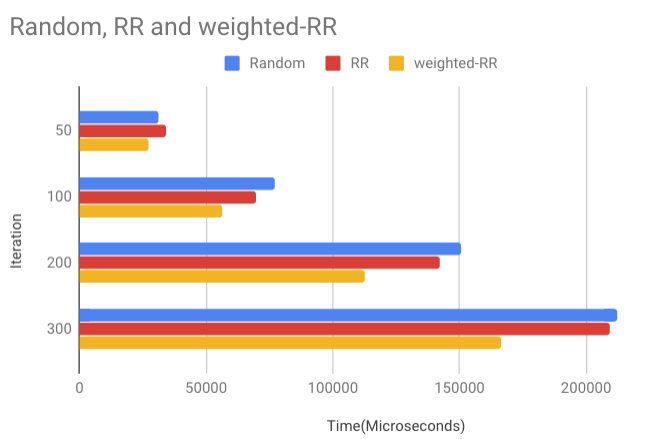
\includegraphics[width=\linewidth]{4.png}
\caption{Turn Around Time with different packet size \label{fig:8}}
\end{figure}


\begin{figure}[ht!]
\centering
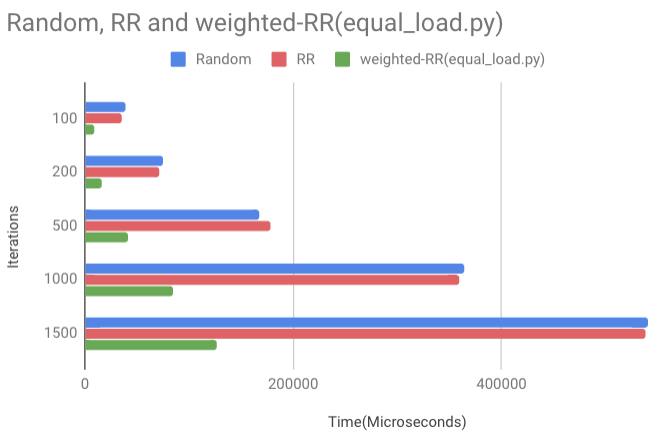
\includegraphics[width=\linewidth]{6.png}
\caption{Turn Around Time with same packet size \label{fig:10}}
\end{figure}

\section{CONCLUSIONS}
\label{sec:conclusion}

Here we have implemented strategy of load balancing using POX controller that works on the principle of SDN. Network is simulated using mininet. We simulated different strategies like random, round robin, weighted round robin and least connections algorithm. The results of our simulation show that weighted round robin out performs all other mentioned algorithms. Random algorithm was giving quite close performance to round-robin because of least number of servers(i.e. 3 in our case). The limitation of our weighted round robin is that we have assumed that initially either we know the link delay or server capacity. This parameter helps to calculate threshold for weighted round robin. We have also assumed the channel/bandwidth of same capacity and error free.

\section{Future Scope}
\label{sec:conclusion}

In this paper, while implementing Random algorithm we assumed all bandwidth have same capacity and they are error free. In future it can be considered as challenge to improve load balancing algorithm. Average response time \& Turn around time was considered as performance metric, but there can be other parameters like bandwidth/channel utilization, Server utilization, ..etc. In weighted-RR, we were not able to come up with relation between link-delay to threshold, so in future it can be improved based on a machine learning statistics result.

 
\addtolength{\textheight}{-12cm}   % This command serves to balance the column lengths
                                  % on the last page of the document manually. It shortens
                                  % the textheight of the last page by a suitable amount.
                                  % This command does not take effect until the next page
                                  % so it should come on the page before the last. Make
                                  % sure that you do not shorten the textheight too much.

%%%%%%%%%%%%%%%%%%%%%%%%%%%%%%%%%%%%%%%%%%%%%%%%%%%%%%%%%%%%%%%%%%%%%%%%%%%%%%%%



%%%%%%%%%%%%%%%%%%%%%%%%%%%%%%%%%%%%%%%%%%%%%%%%%%%%%%%%%%%%%%%%%%%%%%%%%%%%%%%%



%%%%%%%%%%%%%%%%%%%%%%%%%%%%%%%%%%%%%%%%%%%%%%%%%%%%%%%%%%%%%%%%%%%%%%%%%%%%%%%%


\begin{thebibliography}{99}
\bibitem{c1} D. Kreutz, F. M. V. Ramos, P. E. Verıissimo, C. E. Rothenberg, S. Azodolmolky, S. Uhlig, ``Software Defined Networking : A Comprehensive Survey," Proceedings of the IEEE, Vol. 103, No. 1, January 2015.
\bibitem{c2} Wen-Hwa Liao, Ssu-Chi Kuai and Cheng-Hsiu Lu, ``Dynamic Load-Balancing Mechanism for Software-Defined Networking," {\it International Conference on Networking and Network Applications}, 2016.
\bibitem{c3} Sukhveer Kaur, Japinder Singh, Krishan Kumar and Navtej Singh Ghumman, ``Round-Robin Based Load Balancing in Software Defined Networking," Institute of Electrical and Electronics Engineers IEEE, 2015.
\bibitem{c4} Saket Bhelekar, Mrdvika Iyer, Gargee Mehta and Sheetal Chaudhari, ``Dynamic Load Balancing Strategy in Software-Defined Networking," International Conference on Trends in Electronics and Informatics ICEI, 2017.
\bibitem{c5} Walber Jose Adriano Silva, Kelvin Lopes Dias, Djamel Fawzi Hadj Sadok, ``A Performance Evaluation of Software Defined Networking Load Balancers Implementations,"Institute of Electrical and Electronics Engineers IEEE, 2017.
\end{thebibliography}
\end{document}
